\documentclass{article}
\usepackage[margin=0.8in]{geometry}
\usepackage{amsmath}
\usepackage{subfigure}
\usepackage{graphicx}
\usepackage{wasysym}

\title{Conceptual Design Report \\
\large AUToronto AutoDrive GUI}
\author{Team RED}
\date{March 25, 2019}
\begin{document}
\maketitle

\section{Objectives}

This project is aimed to develop a graphical user interface (GUI) to visualize autonomous vehicle data to help monitoring, debugging, and demoing the auto-drive system.

Data to be visualized include: a) raw sensor data, e.g. locations coming from GPS and IMU, and camera images; b) preprocessed data from the control system, e.g. planned path , and recognized objects; c) prior knowlwdge, e.g. a 3D model of our hosting vehicle, and a map of the environment where it is running in. One of the major goals is to create a pipeline from the auToronto core system to the rendering engine of our choice, and enable data visualization in a well organized and maintainable way.

\section{System Architecture}

\begin{figure}[htb]
  \centering
  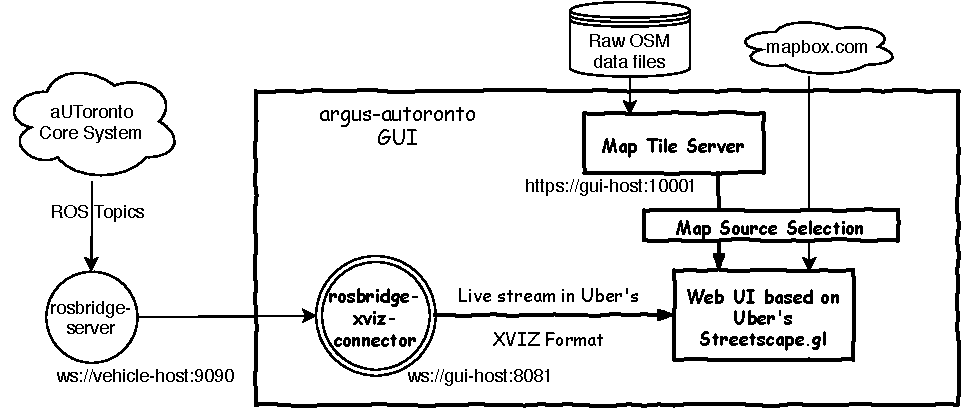
\includegraphics[width=0.7\linewidth]{argus-overview.pdf}
  \caption{System Architecture \cite{github}}
  \label{fig:sys-arch}
\end{figure}

\subsection{Competing Approaches and Design Choices}

In the design phase (Januray, 2019) we reviewed several GUI solutions for other self driving systems, such as Google's Waymo, Baidu's Apollo and Uber. Among those solutions, only Apollo was open-sourced however their documentation was very limited. We therefore decided to write our own rendering system with Unity 3D, a leading 3D game engine with \verb!C#! as its programming language and capable of cross compiling for Linux.

However, with Uber open-sourcing their GUI solution in Feburary 19, 2019 \cite{ubernews}, writing our own rendering logic became less attractive since Uber's solution has the following advantages: a) Professionally implemented and documented by a major company; b) Based on web technologies, therefore easily customizable and easy to use with only a browser as a rendering client.

The web based Uber solution only provides javascript bindings and websocket streaming; nevertheless, we needed a way to pipe our data from ROS systems into the frontend. Fortunately, ROS community has an open-source package called rosbridge \cite{rosbridge} that exposes ROS topics via websocket in JSON format. Though rosbridge has its own formatting that differs with Uber, the websocket API enables easy format conversion in javascript. For these reasons, we use this approach in our final design.

\section{Technical Solution}

As shown in Figure \ref{fig:sys-arch}, our GUI system consistes of 4 main parts:

\textbf{Web UI}: a web application built with Uber's streetscape.gl \cite{streetscapegl}, which is a WebGL and React based visualization client package and a part of Uber's open-source solution mentioned in previous section. It runs in a browser, and consumes data over a websocket connection to a XVIZ data streaming server. 

\textbf{rosbridge-xviz-connector}: A data proxy server that reads from rosbridge-server and serves data in XVIZ format. It is built with the rosbridge client package and the XVIZ server package. XVIZ is another part in the Uber solution that defines a protocol to stream autonomous vehicle data and also provides a collection of libraries that implement the protocol. The core logic of the rosbridge-xviz-connector is to cache and synchronize the data streams coming from the rosbridge server that provides different ROS topics. It then converts data format to XVIZ and serves data to the Web UI.

\textbf{rosbridge-server and aUToronto Core system}: we use rosbridge to get data from the core control system running on ROS and pipe data through a websocket connection to the rosbridge-xviz-connector.

\textbf{Map Tile Server}: the original streetscape.gl UI uses mapbox.com as its default map provider. However, with a need for customized and more accurate map data, we use an open-source tool called TileServerGL \cite{vectortile1} to render maps from raw map data files in OSM (OpenStreetMap) format. Figure \ref{fig:map-flow} describes the flow to generate vector tiles from raw OSM data. Vector tiles contain vector data instead of pixel image tiles, with geometries and metadata — like road names, place names, house numbers — in a compact, structured format. Vector tiles are rendered only when requested by a client, in this case our Web UI running in a browser. 

\begin{figure}[htb]
  \centering
  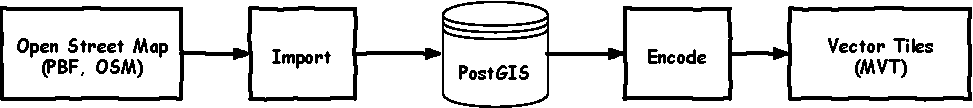
\includegraphics[width=0.8\linewidth]{map-data-flow.pdf}
  \caption{Workflow to Create Vector Tiles from OSM Files}
  \label{fig:map-flow}
\end{figure}

\section{Progress and Results}

\begin{figure}[hb]
  \centering
  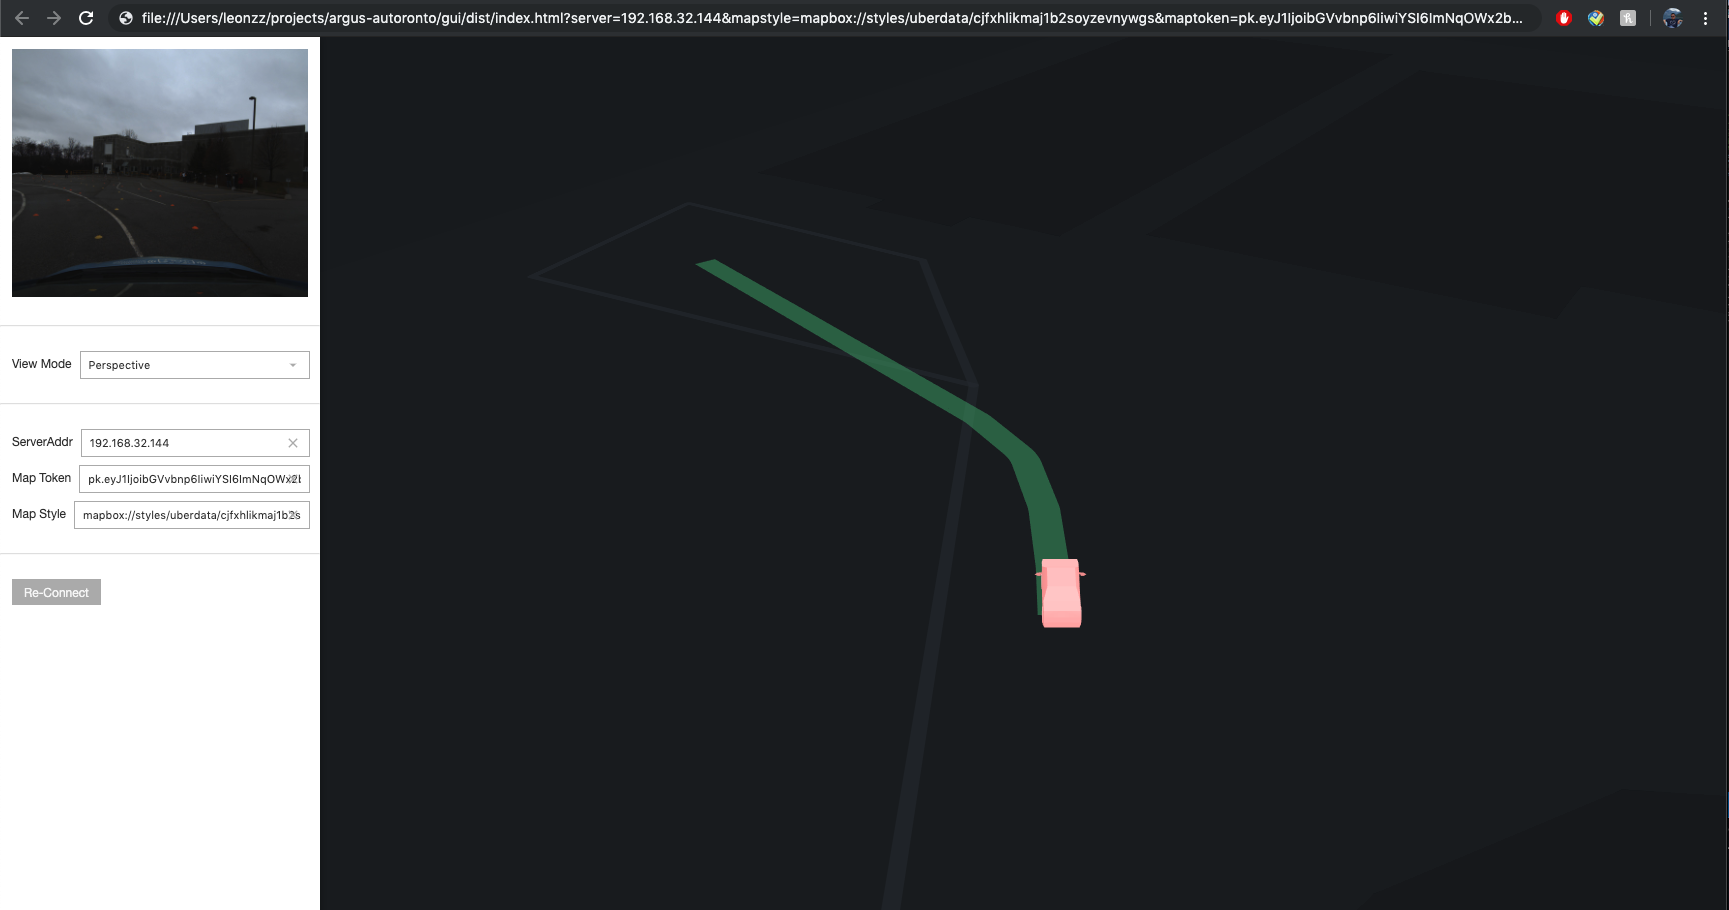
\includegraphics[width=0.7\linewidth]{screenshot.png}
  \caption{Screenshot of GUI Running - A Work in Progress}
  \label{fig:screenshot}
\end{figure}

We have developed our code (available in github \cite{github}) to implement the data pipeline. The system is able to show a vechile moving in a map served by our own map tile server. Visualizations of planned path and camera images are also in progress.

\begin{thebibliography}{7}

\bibitem{github}
Team RED, AER1514 Winter 2019, Github Repo: https://github.com/leonzz/argus-autoronto

\bibitem{rosbridge}
ROS.org, \textit{Rosbridge: JSON API to ROS functionality for non-ROS programs}, http://wiki.ros.org/rosbridge\_suite

\bibitem{ubernews}
Uber ATG, \textit{Introducing AVS, an Open Standard for Autonomous Vehicle Visualization from Uber}, https://eng.uber.com/avs-autonomous-vehicle-visualization/

\bibitem{xviz}
Uber ATG, \textit{XVIZ - A Protocol for Real-Time Transfer and Visualization of Autonomy Data}, https://github.com/uber/xviz

\bibitem{streetscapegl}
Uber ATG, \textit{Streetscape.gl Visualization Toolkit}, Online: https://github.com/uber/streetscape.gl

\bibitem{vectortile1}
Klokan Technologies GmbH, \textit{TileServer GL, An open-source map server made for vector tiles}, Online: http://tileserver.org/

\bibitem{vectortile2}
MapBox, \textit{Map Style Specification} Online: https://docs.mapbox.com/mapbox-gl-js/style-spec


\end{thebibliography}

\end{document}